\documentclass[12px]{article}
\usepackage{amsmath}
\usepackage{amsthm}
\usepackage{mdframed}
\usepackage{amssymb}
\usepackage{nicematrix}
\usepackage{amsfonts}
\usepackage{tcolorbox}
\tcbuselibrary{theorems}
\usepackage{xcolor}
\usepackage{cancel}

\newtheoremstyle{break}
  {1px}{1px}%
  {\itshape}{}%
  {\bfseries}{}%
  {\newline}{}%
\theoremstyle{break}
\newtheorem{theo}{Teorema}
\theoremstyle{break}
\newtheorem{lemma}{Lemma}
\theoremstyle{break}
\newtheorem{defin}{Definizione}
\theoremstyle{break}
\newtheorem{propo}{Proposizione}
\theoremstyle{break}
\newtheorem*{dimo}{Dimostrazione}
\theoremstyle{break}
\newtheorem*{es}{Esempio}

\newenvironment{dimo}
  {\begin{dimostrazione}}
  {\hfill\square\end{dimostrazione}}

\newenvironment{teo}
{\begin{mdframed}[linecolor=red, backgroundcolor=red!10]\begin{theo}}
  {\end{theo}\end{mdframed}}

\newenvironment{nome}
{\begin{mdframed}[linecolor=green, backgroundcolor=green!10]\begin{nomen}}
  {\end{nomen}\end{mdframed}}

\newenvironment{prop}
{\begin{mdframed}[linecolor=red, backgroundcolor=red!10]\begin{propo}}
  {\end{propo}\end{mdframed}}

\newenvironment{defi}
{\begin{mdframed}[linecolor=orange, backgroundcolor=orange!10]\begin{defin}}
  {\end{defin}\end{mdframed}}

\newenvironment{lemm}
{\begin{mdframed}[linecolor=red, backgroundcolor=red!10]\begin{lemma}}
  {\end{lemma}\end{mdframed}}

\newcommand{\icol}[1]{% inline column vector
  \left(\begin{smallmatrix}#1\end{smallmatrix}\right)%
}

\newcommand{\irow}[1]{% inline row vector
  \begin{smallmatrix}(#1)\end{smallmatrix}%
}

\newcommand{\matrice}[1]{% inline column vector
  \begin{pmatrix}#1\end{pmatrix}%
}

\newcommand{\C}{\mathbb{C}}
\newcommand{\K}{\mathbb{K}}
\newcommand{\R}{\mathbb{R}}

\graphicspath{{../../images/}}
\begin{document}
	\section{Moto Circolare uniforme}
	\subsection{Velocità}
	Da semplici considerazioni geometriche si ricava la formula
	\[
	\overrightarrow{v} = \begin{cases}
		v_x = R\cos\omega t\\
		v_y = R\sin\omega t
	\end{cases}
	.\] 
	\subsection{Accelerazione}
	Iniziamo prima con il calcolo del modulo
	\[
	|\overrightarrow{a}| = \lim_{\Delta t \rightarrow 0} \frac {|\Delta \overrightarrow{v}|}{\Delta t} = \frac {v2\sin(\frac{\Delta\theta}2)}{\Delta t} \cdot \frac {\Delta\theta}{\Delta\theta} = v\cdot \frac {\Delta\theta}{\Delta t} = v\cdot\omega
	.\] 
	Il modulo del vettore delta della velocità è stato ricavato dalla considerazione geometrica mostrata in figura
	\begin{center}
		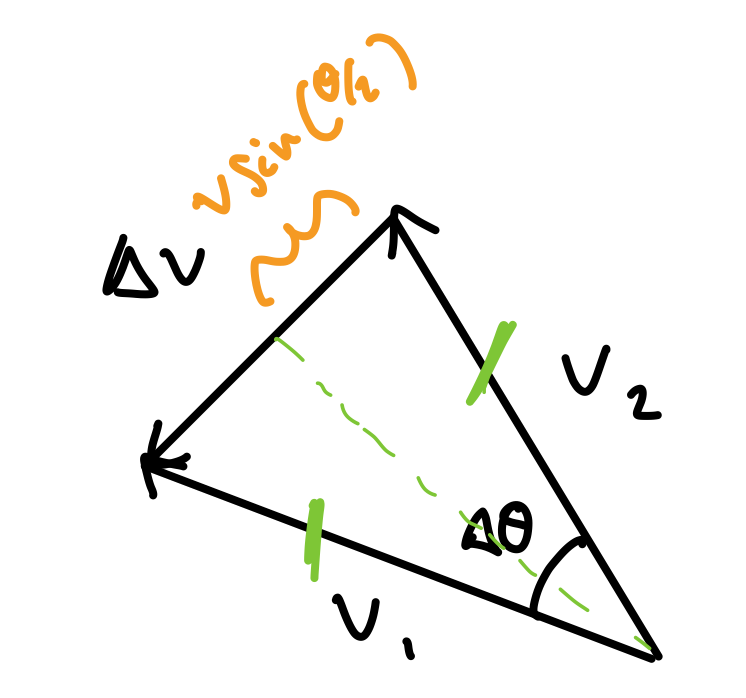
\includegraphics[scale=0.45]{modulo_velocita.jpeg}
	\end{center}
	Per quanto riguarda la direzione del vettore invece, notiamo che il triangolo in figura è isoscele, per tanto gli angoli alla base (che chiameremo per comodità $\alpha$ e $\beta$) sono congruenti, dunque:
	\[
		\alpha \cong \beta \ \ \ \ \alpha + \beta + \Delta\theta = 180 \ \ \ \ \text {se } \Delta\theta \rightarrow 0 \Rightarrow \alpha \cong\beta \cong 90
	.\] 
	Dunque la differenza tra le velocità ha direzione ortogonale a quella del vettore delle velocità, in un moto circolare uniforme questo corrisponde ad un vettore che punta verso il centro. Indicheremo questo versore con $\hat n$\\
	Infine per il calcolo finale del vettore possiamo:
	\[
		\overrightarrow{a} = \diff {\overrightarrow{v}} t = \diff {}t (v \hat v) = \diff v t \hat v + v \diff {\hat v}t = \diff v t \hat v + v\omega \hat n
	.\] 
	Un modo alternativo per scriverlo è:
	\[
		\diff { \overrightarrow{v}} t = \diff v t \hat v + \overrightarrow \omega \times \overrightarrow{v}
	.\]
	Dove il versore $\hat \omega$, è direzionato in modo tale da poter vedere la rotazione in senso antiorario, (uscente se antiorario, entrante se orario)
	Se $|v|$ è  è costante allora
	\[
		\diff { \overrightarrow{v}} t = \overrightarrow\omega \times \overrightarrow{v}
	.\]  è la formula di Poisson\\
	Altrimenti possiamo generalmente scrivere 
	\[
	\overrightarrow{a} = \overrightarrow{a_t} + \overrightarrow{a_n}
	.\] 
	Per indicare la componente tangenziale ($a_t$) e normale ($a_n$) del moto.\\
	Troveremo queste due componenti in moti di piani di traiettoria qualsiasi, difatti definiamo:
	\begin{defi}[Cerchio osculatore]
		Il cerchio osculatore è il cerchio che meglio approssima la traiettoria in un determinato punto $P$.
	\end{defi}
Grazie a questo cerchio osculatore possiamo trattare ogni istante di una traiettoria qualsiasi come se si muovesse su un pezzo di questo cerchio con velocità tangenziale $\overrightarrow{v}$ in $P$. In questo senso il moto coincide con un moto circolare su un cerchio di raggio  $R$ pari al raggio del cerchio osculatore, con velocità angolare istantanea $\omega = \frac v R$, il vettore dell'accelerazione normale invece:
 \[
	 \overrightarrow{a_n} = \frac { v^2}R\hat n = v\omega \hat n
.\]  
Ovviamente avendo l'accelerazione e la velocità in un istante di tempo specificato possiamo ricavare la legge oraria
\end{document}
